\chapter{序論}
\label{chapter1}
宇宙マイクロ波背景放射(Cosmic Microwave Background; CMB)は我々が観測できる宇宙最古の光であり、宇宙初期を知る重要な手がかりとなっている。CMBが持つ温度異方性の観測を基に現代宇宙論の基礎が作られた。しかし、宇宙初期には現在の理論では説明できない物理現象が存在し、これを説明する有力な理論としてインフレーション理論が提唱されている。CMBの偏光にインフレーションの痕跡が残ると考えられており、様々なCMB観測実験が始動している。また、CMBの偏光観測はニュートリノ質量和に対する制限を与えられ、素粒子物理学にも大きな影響を持つ。この章では、CMBとそれを取り巻く宇宙論の関係について述べる。

\section{CMBの温度異方性と現代宇宙論}
%ビッグバン理論は宇宙初期が高温高密度であり、膨張しながら星や銀河を作り、今に至るという宇宙のシナリオを予言した。ビッグバンの証拠には宇宙膨張を示すハッブルの法則やビッグバン元素合成(Big Bang Nucleosynthesis; BBN\cite{BBN})と呼ばれる初期宇宙の軽元素の生成過程が挙げられる。そしてもう1つの証拠はCMBの周波数スペクトルがほぼ\SI{2.725}{K}の黒体放射のスペクトルと一致するという観測事実\cite{2725}である。このことで宇宙初期は熱平衡状態だったことが証明された。

%宇宙初期は高温高密度であり、バリオン物質がイオン化しており、光子は電子と頻繁に散乱される不透明な状況であった。宇宙が膨張して冷えていくにつれてイオンの中性化が進み、電子の個数密度も減少していく。宇宙の温度がおよそ\SI{2970}{K}、宇宙年齢にしておよそ\SI{37}{万年}で光子と電子の散乱率がハッブルパラメータ(宇宙の膨張率)よりも小さくなり、光は散乱されずに真っすぐ進むようになる。この時期を``宇宙の晴れ上がり''または``最終散乱時刻''と呼ぶ\footnote{宇宙の晴れ上がりは光子と電子の散乱率がハッブルパラメータより小さくなる時期、最終散乱時刻はCMB光子が電子と最後に散乱する時刻として定義されるため厳密には異なる時刻を表すが、ほぼ同時刻とみなしてもよい}。我々観測者は最終散乱時刻に対応する``最終散乱面''に囲まれており、そこから散乱されることなく届くCMB光子を観測することができる。

\subsection{CMBの温度異方性}
ビッグバン理論は宇宙初期が高温高密度であり、膨張しながら星や銀河を作り、今に至るという宇宙のシナリオを予言した。ビッグバンの証拠には宇宙膨張を示すハッブルの法則やビッグバン元素合成(Big Bang Nucleosynthesis; BBN\cite{BBN})と呼ばれる初期宇宙の軽元素の生成過程が挙げられる。そしてもう1つの証拠はCMBの周波数スペクトルがほぼ\SI{2.725}{K}の黒体放射のスペクトルと一致するという観測事実\cite{2725}である。このことで宇宙初期は熱平衡状態だったことが証明された。

宇宙初期は高温高密度であり、バリオン物質がイオン化しており、光子は電子と頻繁に散乱される不透明な状況であった。宇宙が膨張して冷えていくにつれてイオンの中性化が進み、電子の個数密度も減少していく。宇宙の温度がおよそ\SI{2970}{K}、宇宙年齢にしておよそ\SI{37}{万年}で光子と電子の散乱率がハッブルパラメータ(宇宙の膨張率)よりも小さくなり、光は散乱されずに真っすぐ進むようになる。この時期を``宇宙の晴れ上がり''または``最終散乱時刻''と呼ぶ\footnote{宇宙の晴れ上がりは光子と電子の散乱率がハッブルパラメータより小さくなる時期、最終散乱時刻はCMB光子が電子と最後に散乱する時刻として定義されるため厳密には異なる時刻を表すが、ほぼ同時刻とみなしてもよい。}。我々観測者は最終散乱時刻に対応する``最終散乱面''に囲まれており、そこから散乱されることなく届くCMB光子を観測することができる。

CMBがほぼ\SI{2.725}{K}の黒体放射のスペクトルを持つと同時にわずかな温度異方性を持つことも発見された。ある空の1点でのCMB温度を$T(\theta,\phi)$とする。全方向で平均した温度は
\begin{equation}
  \langle T \rangle = \frac{1}{4\pi}\int T(\theta,\phi)\sin\theta d\theta d\phi = \SI{2.725}{\mathrm{K}}
\end{equation}
である。この空の1点$(\theta,\phi)$における温度揺らぎを
\begin{equation}
  \frac{\Delta T}{T}(\theta,\phi) \equiv \frac{T(\theta,\phi) - \langle T \rangle}{\langle T \rangle}
\end{equation}
と定義する。Planck衛星によって観測された温度揺らぎ\cite{Planck_T}は$\sim \SI{100}{\mu\mathrm{K}}$であり、わずかな温度異方性を示している(図\ref{Planck_T})。

\begin{figure}[htbp]
  \centering
  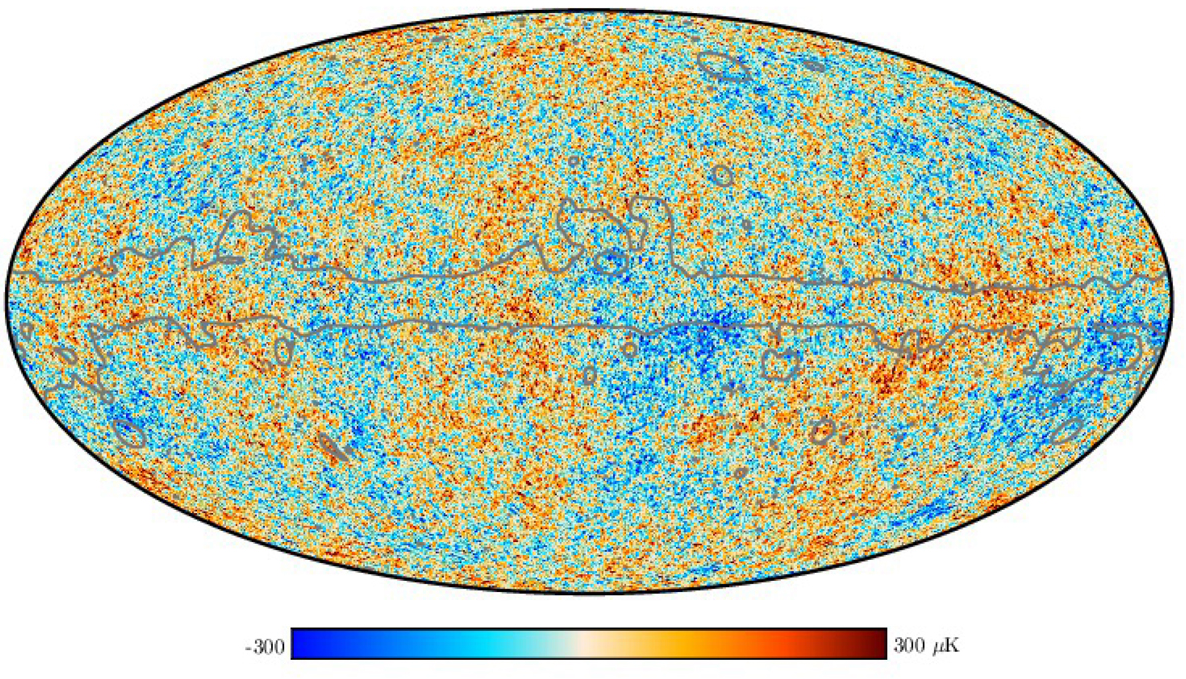
\includegraphics[width=0.85\columnwidth]{2_cosmology/figs/planck_T_map_single.png}
  \caption{Planck衛星によって観測されたCMBの温度異方性のマップ。}
  \label{Planck_T}
\end{figure}
CMB実験ではCMBの観測データと望遠鏡の角度データを用いて図\ref{Planck_T}で示すようなCMBの異方性を表す``マップ(強度分布図)''を作成する。このマップを球面調和関数$Y^{m}_{\ell}(\theta,\phi)$で展開してパワースペクトル($C_{\ell}$)作成することで、宇宙論パラメータを求めることができる。空(天球面上)の$(\theta,\phi)$(図\ref{kyuuzahyou})に対して単位ベクトル$\hat{n}$を
\begin{equation}
  \hat{n} \equiv (\sin\theta\cos\phi,\sin\theta\sin\phi,\cos\theta)
\end{equation}
と定義する。
\begin{figure}[htbp]
  \centering
  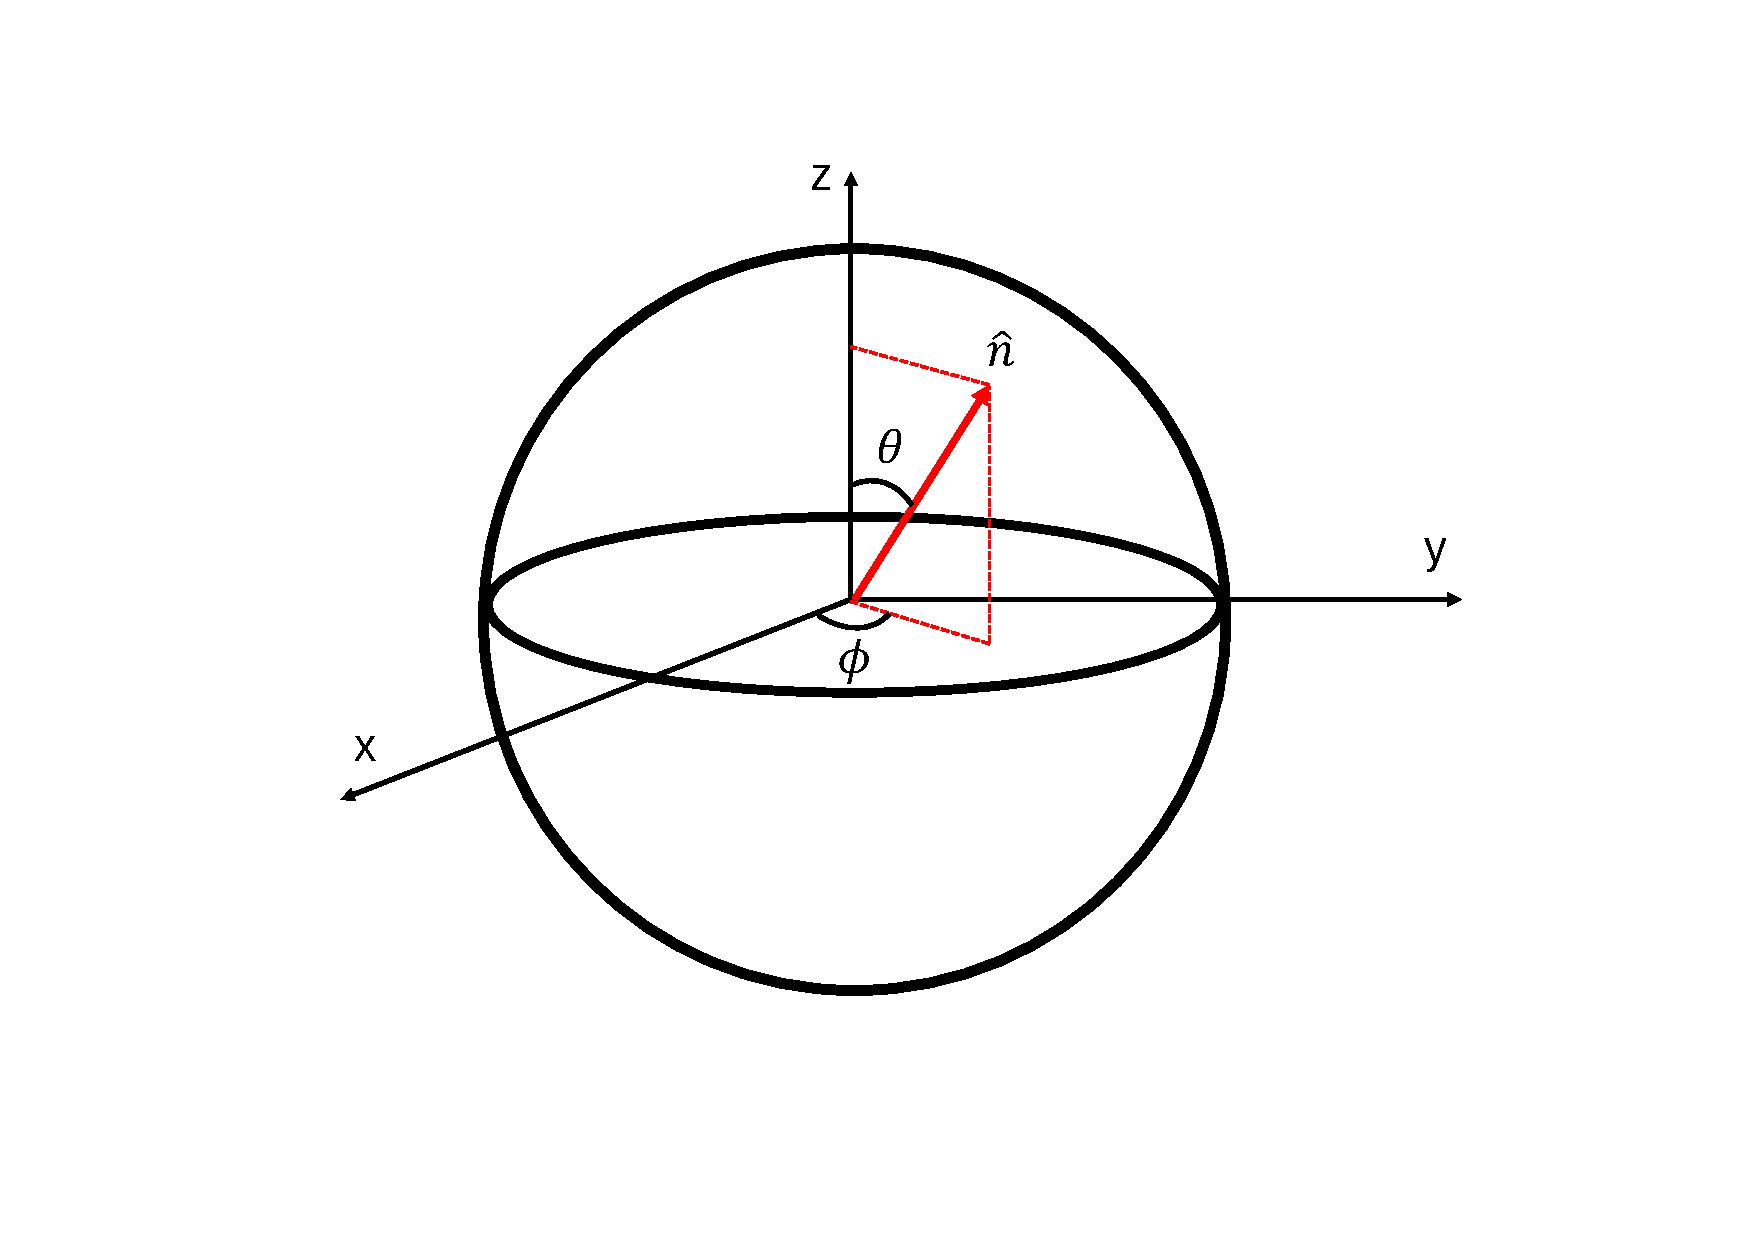
\includegraphics[width=0.5\columnwidth]{2_cosmology/figs/kyuuzahyou.pdf}
  \caption{天球面の座標。}
  \label{kyuuzahyou}
\end{figure}
この時、CMBの温度異方性$\Delta T(\hat{n})\equiv T(\hat{n}) - \langle T \rangle$を球面調和関数で
\begin{equation}
  \Delta T(\hat{n}) = \sum_{\ell=1}^{\infty}\sum_{m=-\ell}^{\ell}a_{\ell m}Y^{m}_{\ell}(\hat{n})
\end{equation}
と展開する。ここで、$a_{\ell m}$は展開係数である。また、$m$は揺らぎの方向を決め、$\ell$は揺らぎのスケールの大きさを表す。$\ell$と角度スケール($\delta\theta$)の関係は
\begin{equation}
  \delta\theta = \SI{180}{^{\circ}}/\ell
\end{equation}
と表せる。しかし、展開係数$a_{\ell m}$は添字$m$による座標依存性があるため、パワースペクトル$C_{\ell}$は展開係数$a_{\ell m}$に対して
\begin{equation}
  C_{\ell}\equiv\frac{1}{2\ell+1}\sum_{m=-\ell}^{\ell}a_{\ell m}{a^{\ast}_{\ell m}}
\end{equation}
と定義することで、座標に依らない物理量として扱うことができる。

\subsection{$\Lambda$-CDMモデル}
CMBのパワースペクトルの測定により、$\Lambda$-CDMモデルと呼ばれる宇宙の進化を記述する標準理論が構築された(図\ref{fit_planck})。$\Lambda$-CDMモデルは、6つのパラメータのみで宇宙を記述するもので、$\Lambda$はダークエネルギーに対応するアインシュタインの宇宙定数を表し、CDMは``Cold Dark Matter''を意味する。
\begin{figure}[htbp]
  \centering
  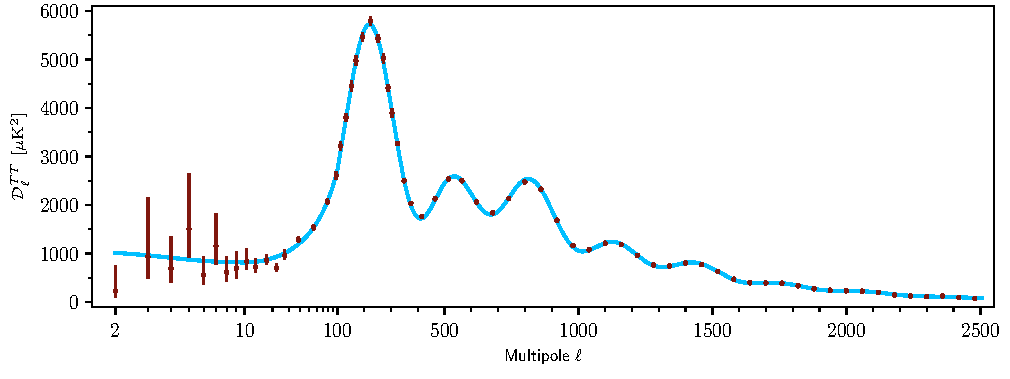
\includegraphics[width=0.85\columnwidth]{2_cosmology/figs/plank_cltt.pdf}
  \caption{Planckの観測から計算されたCMBの温度パワースペクトル\cite{Planck_T}。縦軸の$\mathcal{D}^{TT}_{\ell}$は$\mathcal{D}^{TT}_{\ell} = \frac{\ell(\ell+1)C_{\ell}}{2\pi}$を表す。青の線は$\Lambda$-CDMモデルのベストフィットを表す。}
  \label{fit_planck}
\end{figure}
現在での$\Lambda$-CDMモデルのパラメータを表\ref{6params}にまとめる。
\vspace{2mm}
\begin{table}[htbp]
  \centering
  \caption{Planckの観測から得られた$\Lambda$-CDMモデルの宇宙論パラメータ\cite{Planck_T}。
  これらの値の推定にはCMBの偏光、lensingのパワースペクトル、バリオン音響振動も用いる。}
  \vspace{2mm}
  \begin{tabular}{l|l}\hline
    $\Omega_{b} h^2$ ~(バリオン密度)& 0.02242 $\pm$ 0.00014 \\
    $\Omega_{c} h^2$ ~(CDM密度)& 0.11933 $\pm$ 0.00091 \\
    $100\theta_{MC}$ ~(最終散乱面の見込み角度) & 1.04101 $\pm$ 0.00029 \\
    $\tau$ ~(再電離期における光学的厚み)& 0.0561 $\pm$ 0.0071 \\
    $ln(10^{10}A_s)$ ~(スカラー型の原始揺らぎの振幅) & 3.047 $\pm$ 0.014 \\
    $n_s$ ~(スカラー型の原始揺らぎのべき係数)& 0.9665 $\pm$ 0.0038 \\ \hline
  \end{tabular}
  \label{6params}
\end{table}

\subsection{地平線問題}

\section{CMBの偏光とインフレーション理論}

\subsection{インフレーション理論}

\subsection{CMBの偏光モード}

\subsection{偏光Bモードの探索状況}

\section{CMBの偏光とニュートリノ質量和}

\subsection{光学的厚み~$\tau$}

\subsection{ニュートリノ質量和との縮退}

\subsection{偏光Eモードと$\tau$}
\label{E_and_tau}
